\documentclass{beamer}
\mode<presentation> {
    \usetheme{Copenhagen} \usecolortheme{whale}
    }
\usepackage{graphicx}
\usepackage{multicol}
\setbeamersize{text margin left=3mm,text margin right=5mm}

\graphicspath{{Images/}}

\title[Assignments 1]{Stima dei Parametri di un modello P-SP}
\author{Lorenzo Rossi Matricola: 0301285}
\begin{document}
\begin{frame}
\titlepage{}
\end{frame}
\begin{frame}
    \begin{columns}[t]
        \begin{column}{.5\textwidth}
            \tableofcontents[sections={1-3}]
        \end{column}
        \begin{column}{.5\textwidth}
            \tableofcontents[sections={4-5}]
        \end{column}
    \end{columns}
\end{frame}
\begin{frame}
    \frametitle{Assignment 1}
    \section{Introduzione}
    Considerato il sistema:
    \begin{equation*}
        \dot{x}=-ax+bu\quad a=1,b=2
    \end{equation*}
    Effettua delle simulazioni per i modelli Parallelo (P) e Serie-Parallelo (SP) e valutare le performance degli algoritmi in presenza di rumori e vari segnali di ingresso. Inoltre, valutare le performance degli algoritmi di stima adattativa considerando che il parametro \( a\) varia come:
    \begin{equation*}
        a=1+0.1\sin(\frac{2\pi t}{24\times 3600})
    \end{equation*}
\end{frame}
\begin{frame}
    \frametitle{Modello Teorico}
    \section{Modello Teorico}
    \begin{minipage}{0.45\textwidth}
        \begin{center}
            \textbf{Modello Parallelo (P)}
            \begin{equation*}
                \dot{\hat{x}}=-\hat{a}\hat{x}+\hat{b}u
            \end{equation*}
            \begin{equation*}
                \dot{\hat{a}}=-(x-\hat{x})\hat{x}
            \end{equation*}
            \begin{equation*}
                \dot{\hat{b}}=-(x-\hat{x})u
            \end{equation*}
        \end{center}
    \end{minipage}
    \begin{minipage}{0.45\textwidth}
        \begin{center}
            \textbf{Modello Parallelo (P)}
            \begin{equation*}
                \dot{\hat{x}}=-a_{m}\hat{x}+(a_{m}-\hat{a})x+\hat{b}u
            \end{equation*}
            \begin{equation*}
                \dot{\hat{a}}=-(x-\hat{x})x
            \end{equation*}
            \begin{equation*}
                \dot{\hat{b}}=-(x-\hat{x})u
            \end{equation*}
        \end{center}
    \end{minipage}
\end{frame}
\begin{frame}
    \frametitle{Simulink - 1}
    \section{Implementazione Simulink}
    \subsection{Modello Parallelo}
    \begin{itemize}
        \item \textbf{Modello Parallelo}
    \end{itemize}
\begin{center}
            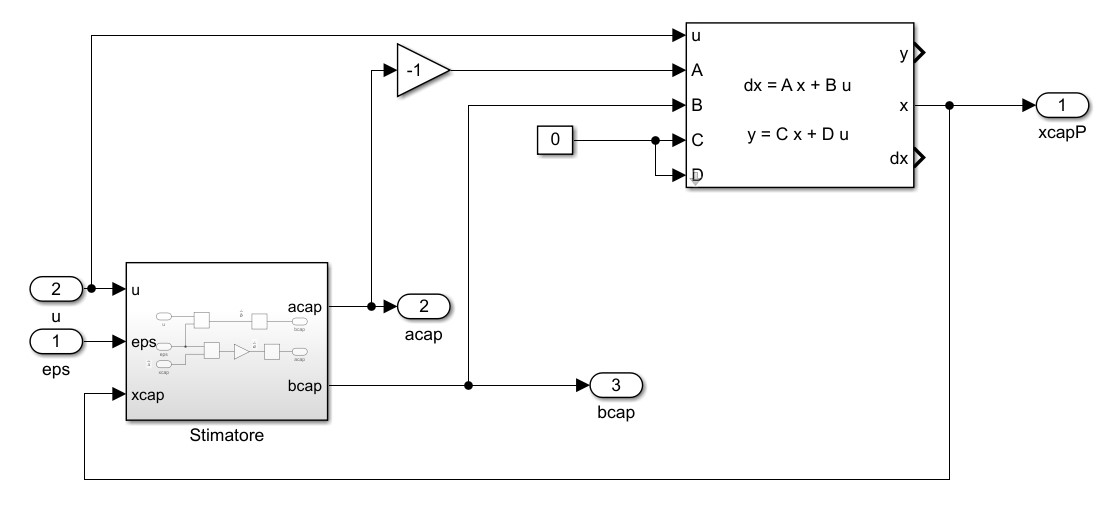
\includegraphics[scale=0.3]{ModelloParallelo.jpg}% chktex 8
        \end{center}
\end{frame}
\begin{frame}
    \frametitle{Simulink - 2}
    \subsection{Stimatore Parallelo}
    \begin{itemize}
        \item \textbf{Stimatore Parallelo}
    \end{itemize}
        \begin{center}
            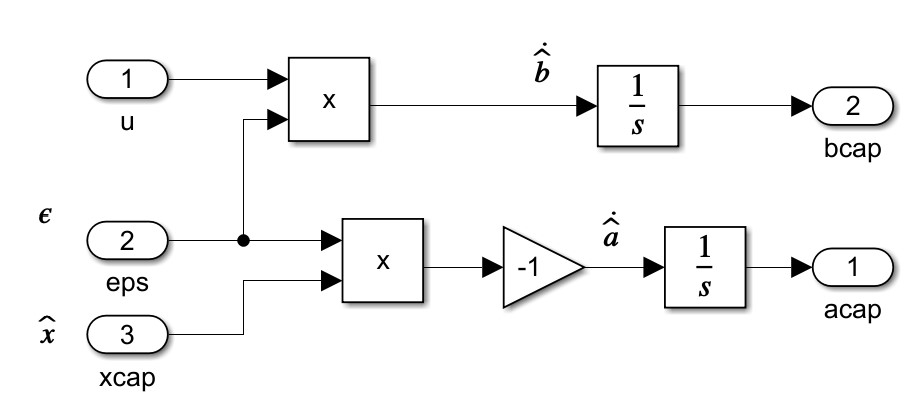
\includegraphics[scale=0.3]{StimatoreParallelo.jpg}% chktex 8
        \end{center}
\end{frame}
\begin{frame}
    \frametitle{Simulink - 3}
    \subsection{Modello Serie-Parallelo}
    \begin{itemize}
        \item \textbf{Modello Serie-Parallelo}
    \end{itemize}
    \begin{center}
        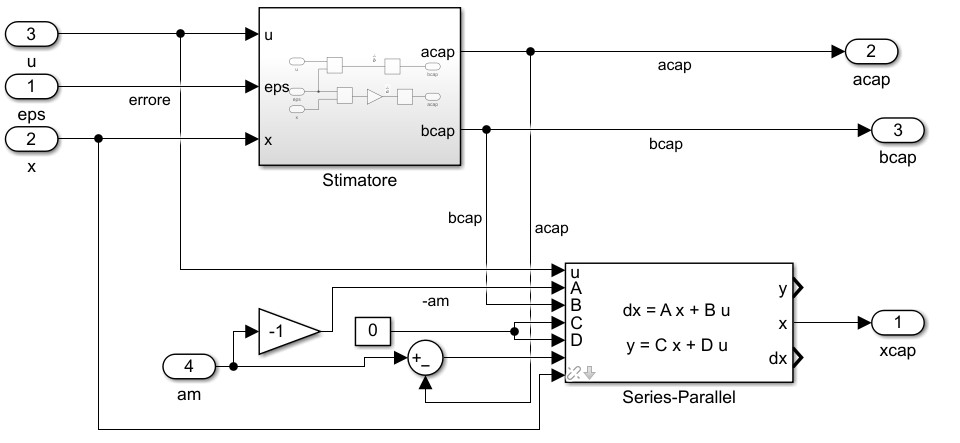
\includegraphics[scale=0.3]{ModelloSerieParallelo.jpg}% chktex 8
    \end{center}
\end{frame}
\begin{frame}
    \frametitle{Simulink - 4}
    \subsection{Stimatore Serie-Parallelo}
    \begin{itemize}
        \item \textbf{Stimatore Serie-Parallelo}
    \end{itemize}
    \begin{center}
        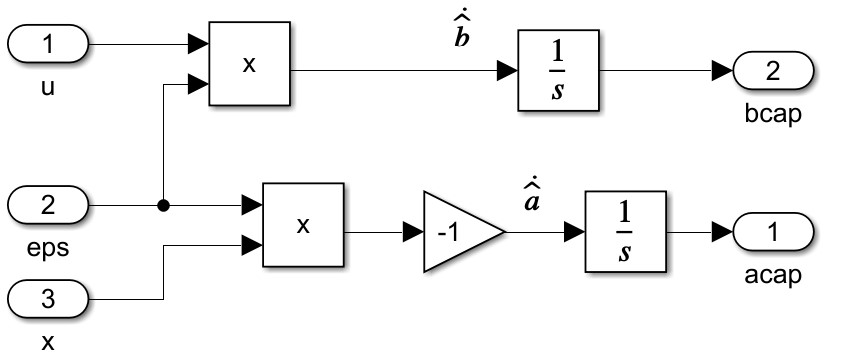
\includegraphics[scale=0.3]{StimatoreSerieParallelo.jpg}% chktex 8
    \end{center}
\end{frame}
\begin{frame}
    \frametitle{Simulink - 4}
    \subsection{Sistema Complessivo}
    \begin{itemize}
        \item \textbf{Sistema Complessivo}
    \end{itemize}
    \begin{center}
        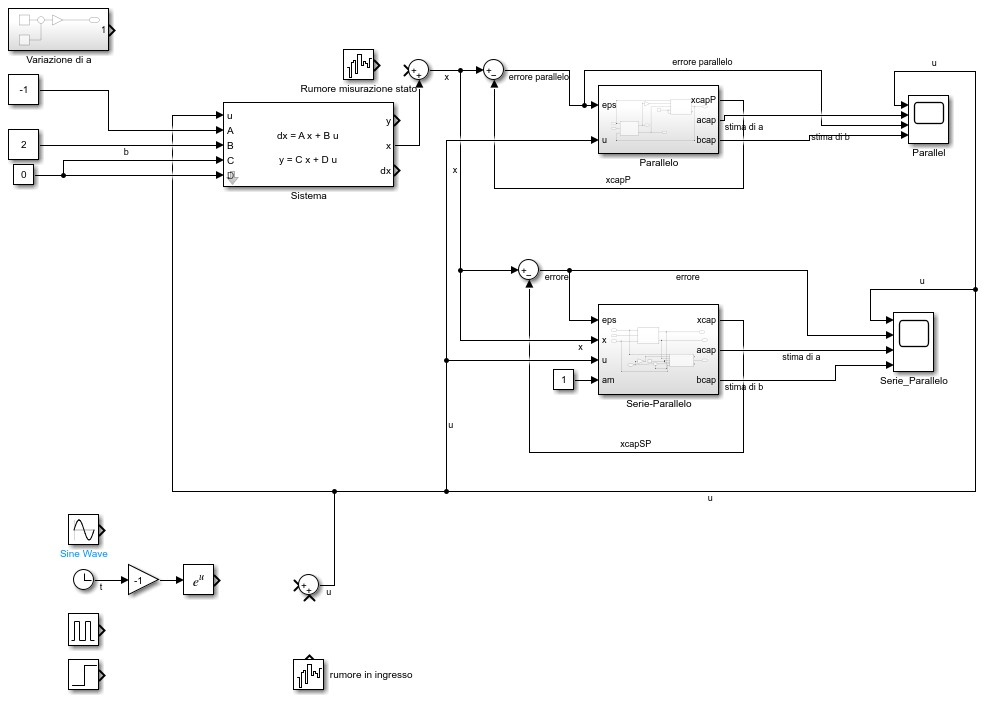
\includegraphics[scale=0.3]{Complessivo.jpg}% chktex 8
    \end{center}
\end{frame}
\begin{frame}
    \frametitle{Analisi}
    \section{Analisi}
       \begin{enumerate}
           \item Gli ingressi scelti per valutare le performance degli algoritmi di stima adattativa sono in ordine:
           \begin{itemize}
               \item Ingresso sinusoidale;
               \item Ingresso esponenziale;
               \item Ingresso a gradino;
               \item Ingresso impulsivo;
               \item Ingresso sinusoidale in presenza di rumore;
           \end{itemize}
           \item Variazione del parametro a valutazione delle performance;
       \end{enumerate}
\end{frame}
\begin{frame}
    \frametitle{Ingresso Sinusoidale}
    \subsection{Ingresso Sinusoidale}
    \begin{tabular}{cc}
            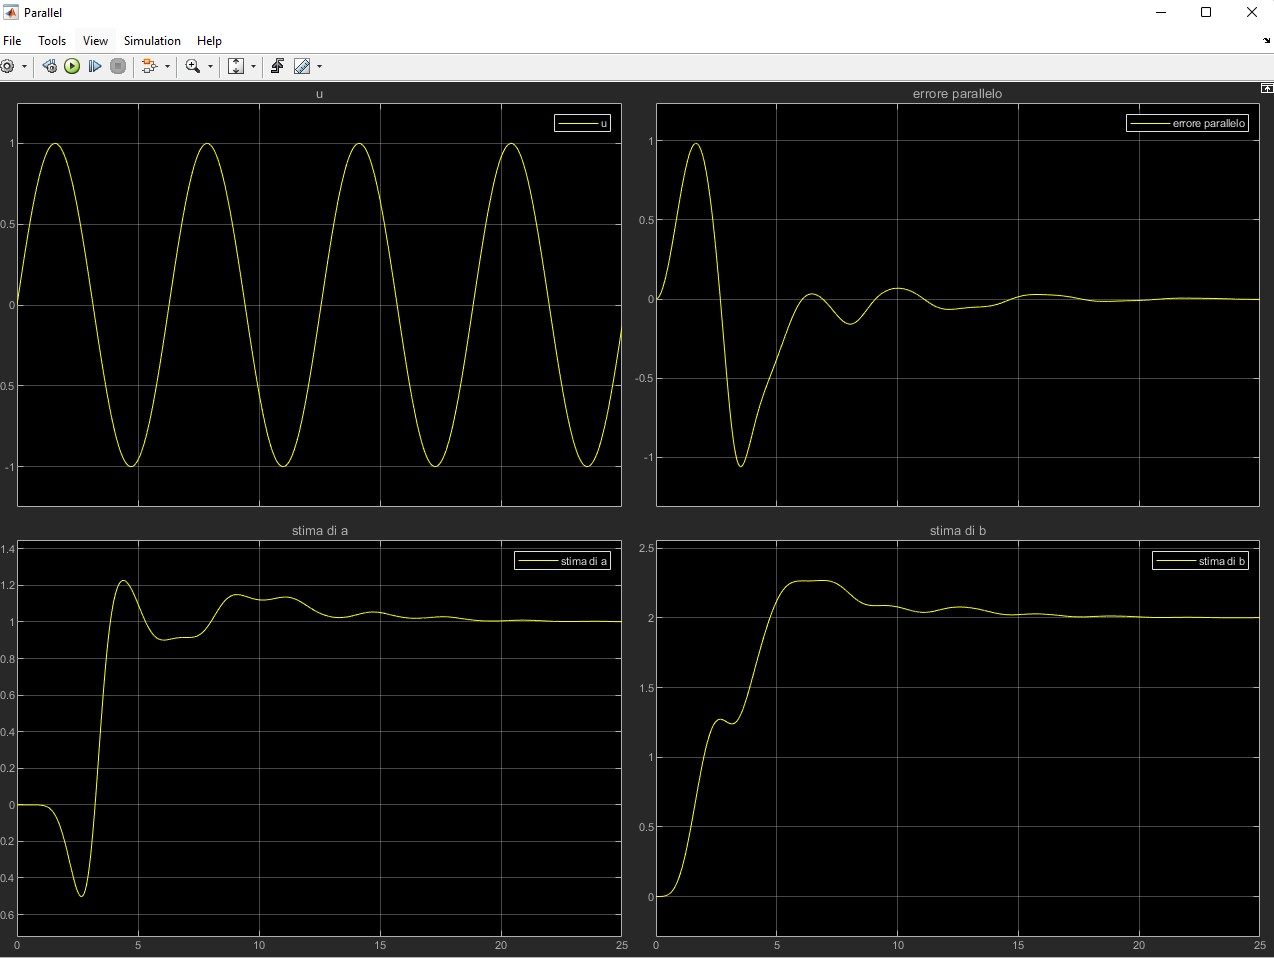
\includegraphics[ scale=0.15]{ScopeSinP.jpg}
        &
            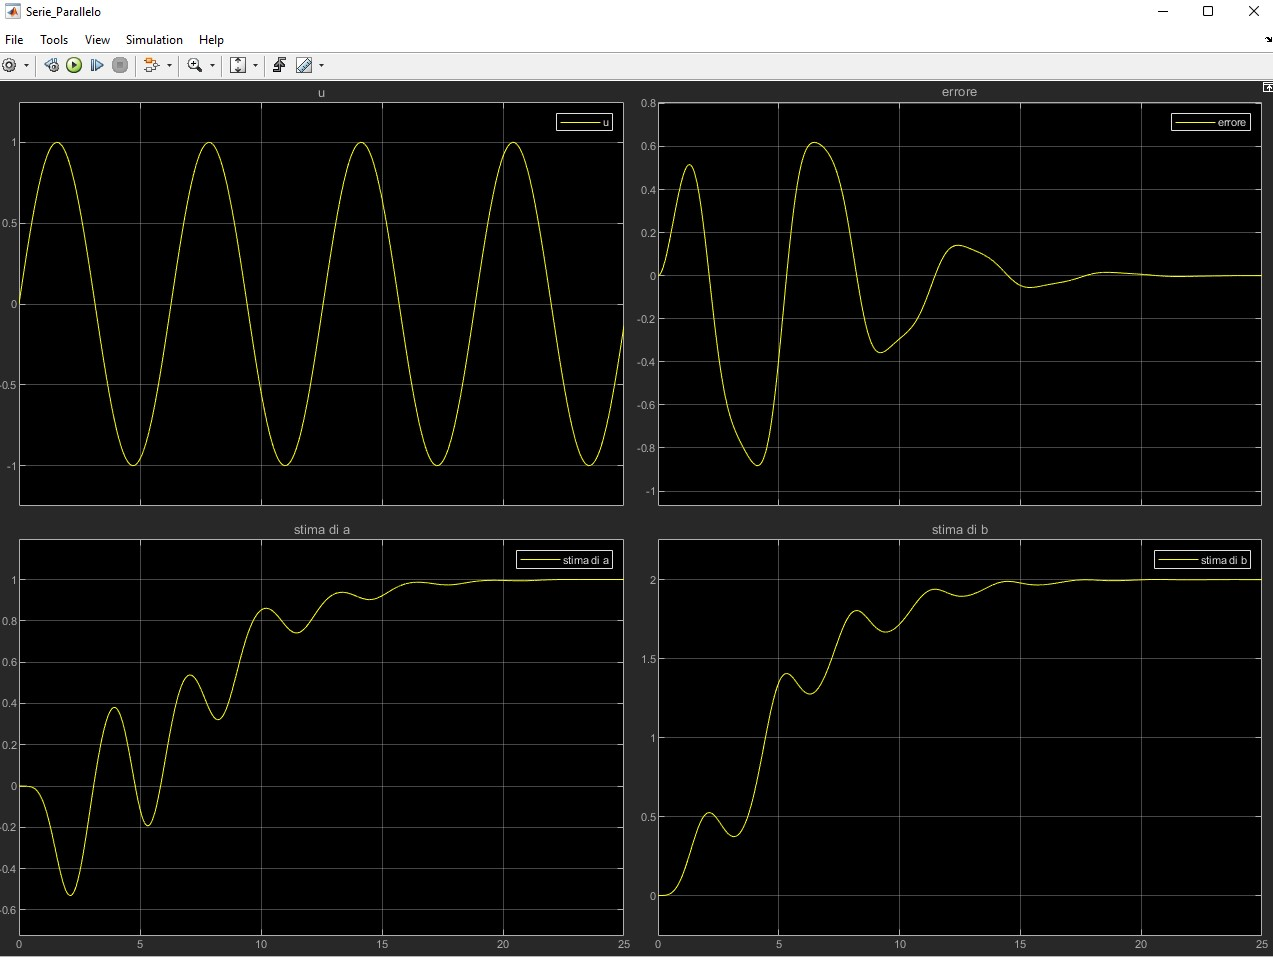
\includegraphics[ scale=0.15]{ScopeSinSP.jpg}
        \\
    \end{tabular}\newline
Entrambi gli algoritmi riescono a stimare correttamente i parametri \(a\) e \(b\) nel tempo di simulazione di 25s. Tuttavia, la stima effettuata dal modello Serie-Parallelo (SP) presenta incertezza dovuta alle numerose oscillazioni nelle stime di a e b.
\end{frame}
\begin{frame}
    \frametitle{Ingresso Esponenziale \(e^{-t}\)}
    \subsection{Ingresso Esponenziale}
    \begin{tabular}{cc}
            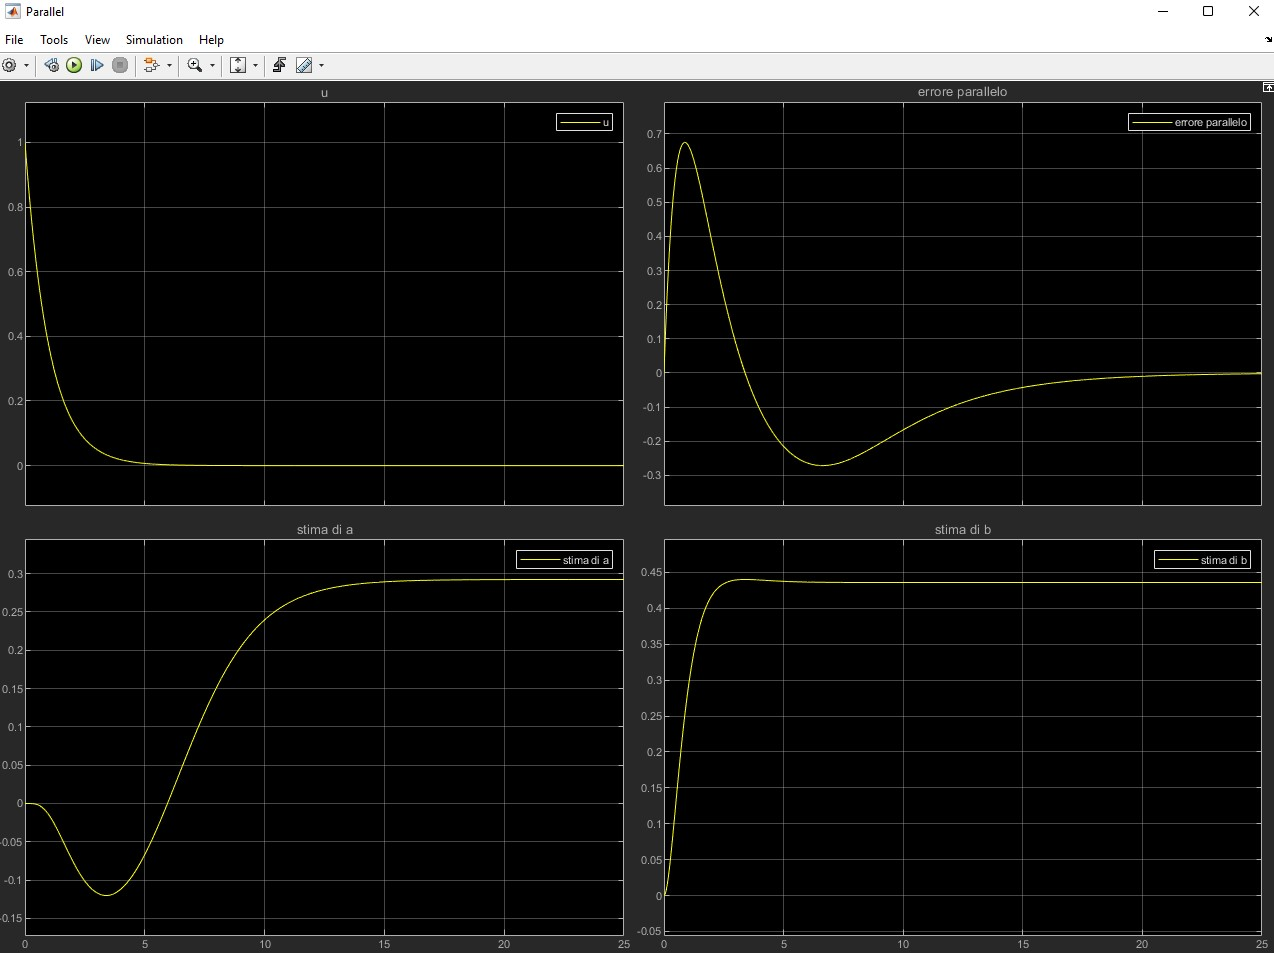
\includegraphics[ scale=0.15]{expP.jpg}
        &
            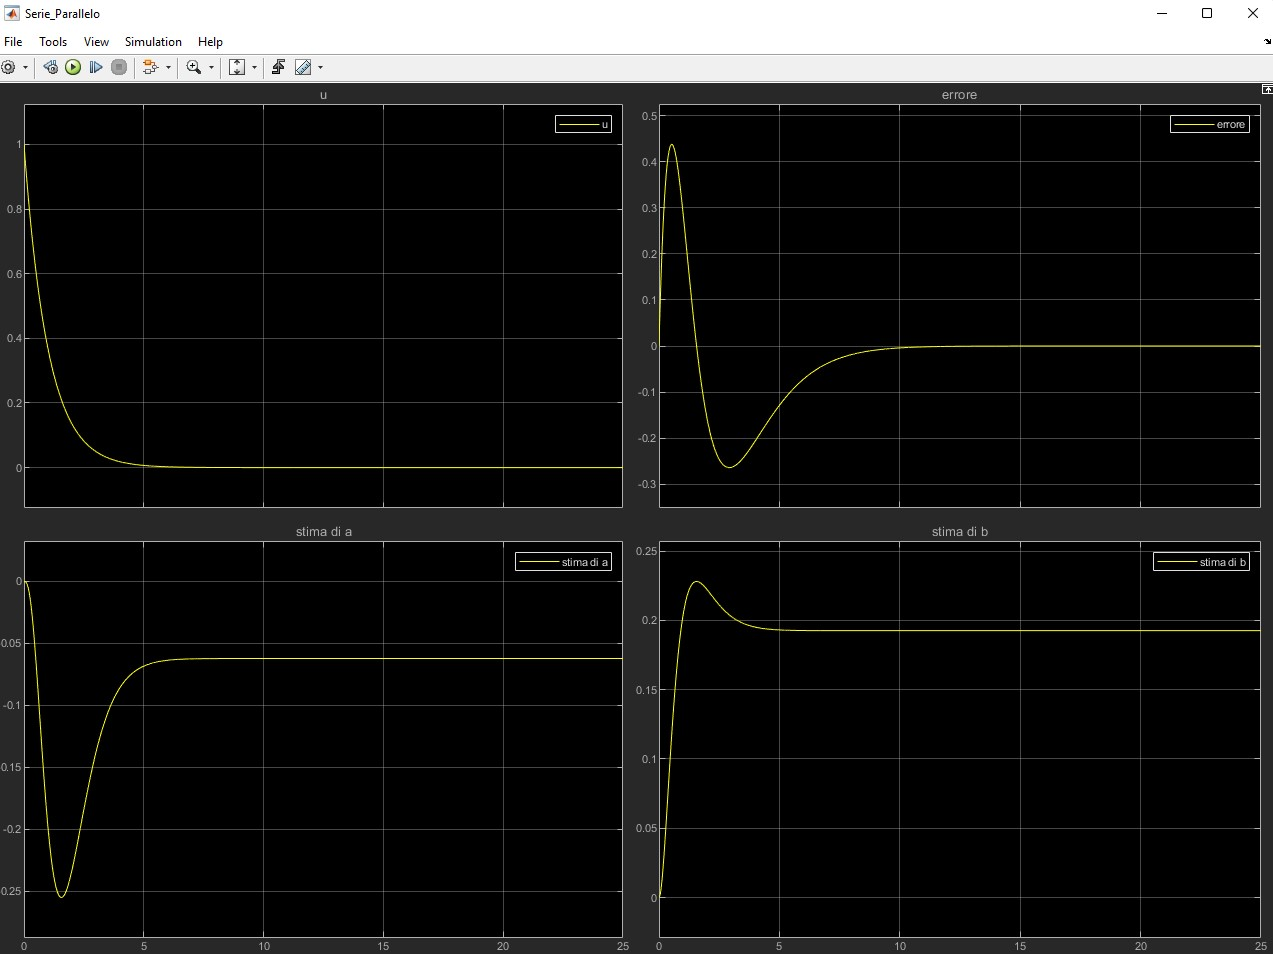
\includegraphics[ scale=0.15]{expSP.jpg}
        \\
    \end{tabular}\newline
Entrambi gli algoritmi non riescono a stimare correttamente i parametri \(a\) e \(b\) nel tempo di simulazione di 25s. La stima effettuata sembra convergere verso i parametri del sistema finché l'azione del controllo \(u=\exp^{-t}\neq 0\).
\end{frame}
\begin{frame}
    \frametitle{Ingresso a gradino }
    \subsection{Ingresso a gradino}
    \begin{tabular}{cc}
            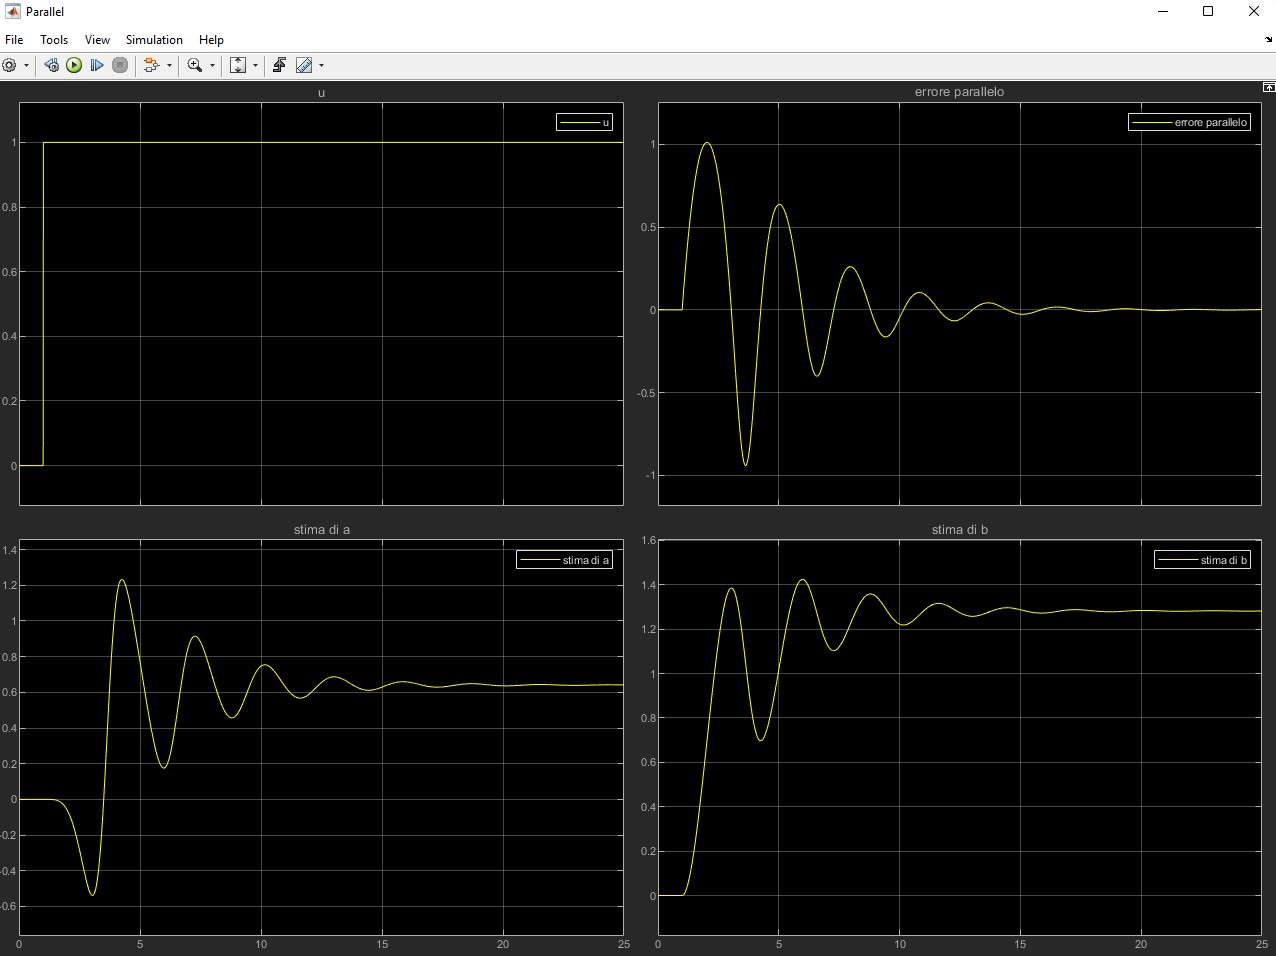
\includegraphics[ scale=0.15]{gradinoP.jpg}
        &
            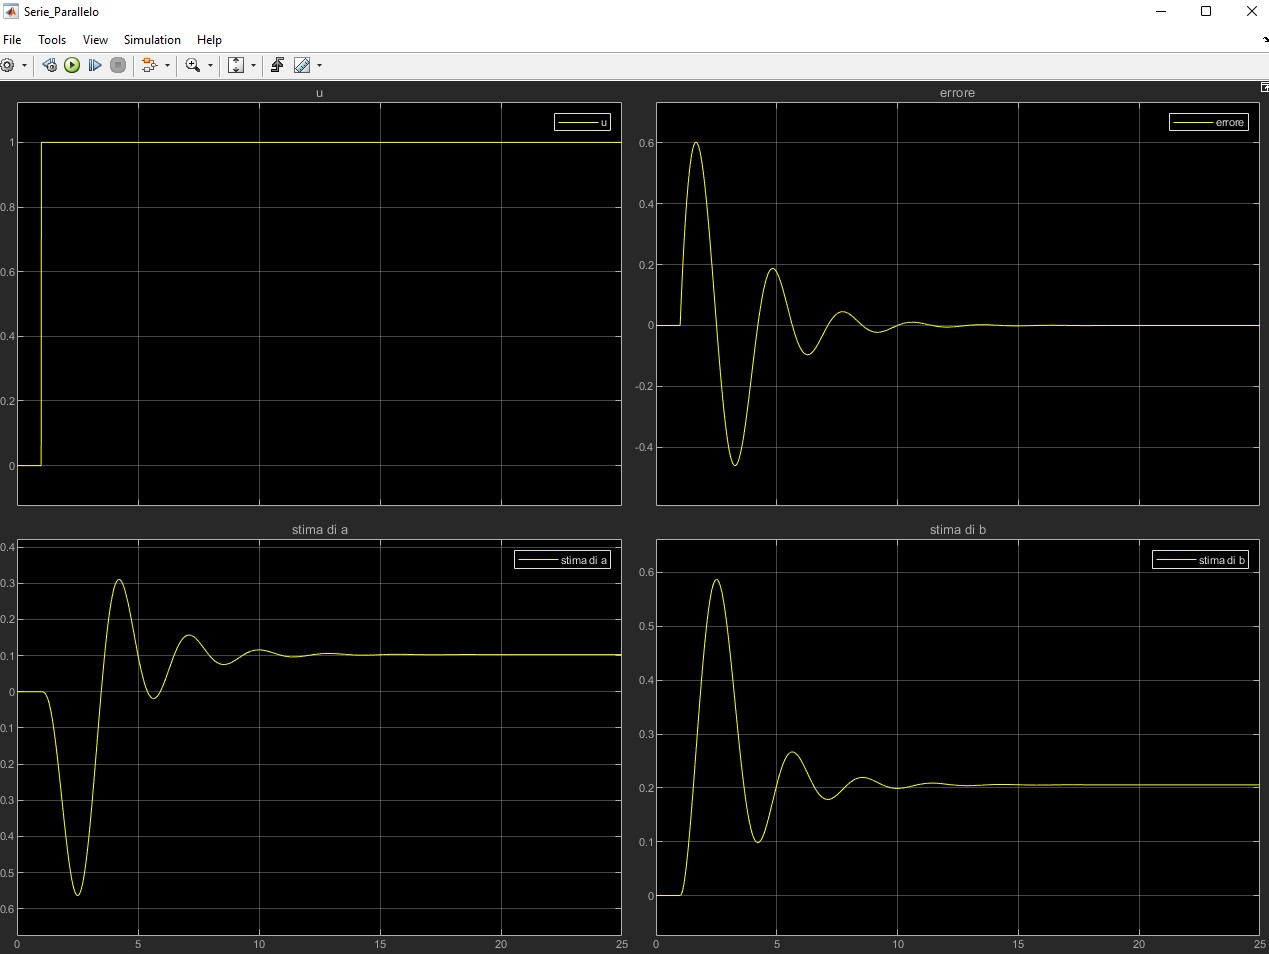
\includegraphics[ scale=0.15]{gradinoSP.jpg}
        \\
    \end{tabular}\newline
Entrambi gli algoritmi non riescono a stimare correttamente i parametri \(a\) e \(b\) nel tempo di simulazione di 25s. Anche aumentando il tempo di simulazione, si vede che il valore delle stime rimane pressoché invariato.
\end{frame}
\begin{frame}
    \frametitle{Ingresso impulsivo}
    \subsection{Ingresso impulsivo}
    \begin{tabular}{cc}
            \includegraphics[ scale=0.15]{impulsoP.jpg}
        &
            \includegraphics[ scale=0.15]{impulsoSP.jpg}
        \\
    \end{tabular}\newline
Con un ingresso di tipo impulsivo, il tempo necessario all'algoritmo di stima adattativa per stimare i valori di \(a\) e \(b\) vengono notevolmente aumentati anche ad arrivare ad 800s.
\end{frame}
\begin{frame}
    \frametitle{Ingresso sinusoidale con rumore in ingresso}
    \subsection{Ingresso sinusoidale con rumore in ingresso}
    \begin{tabular}{cc}
            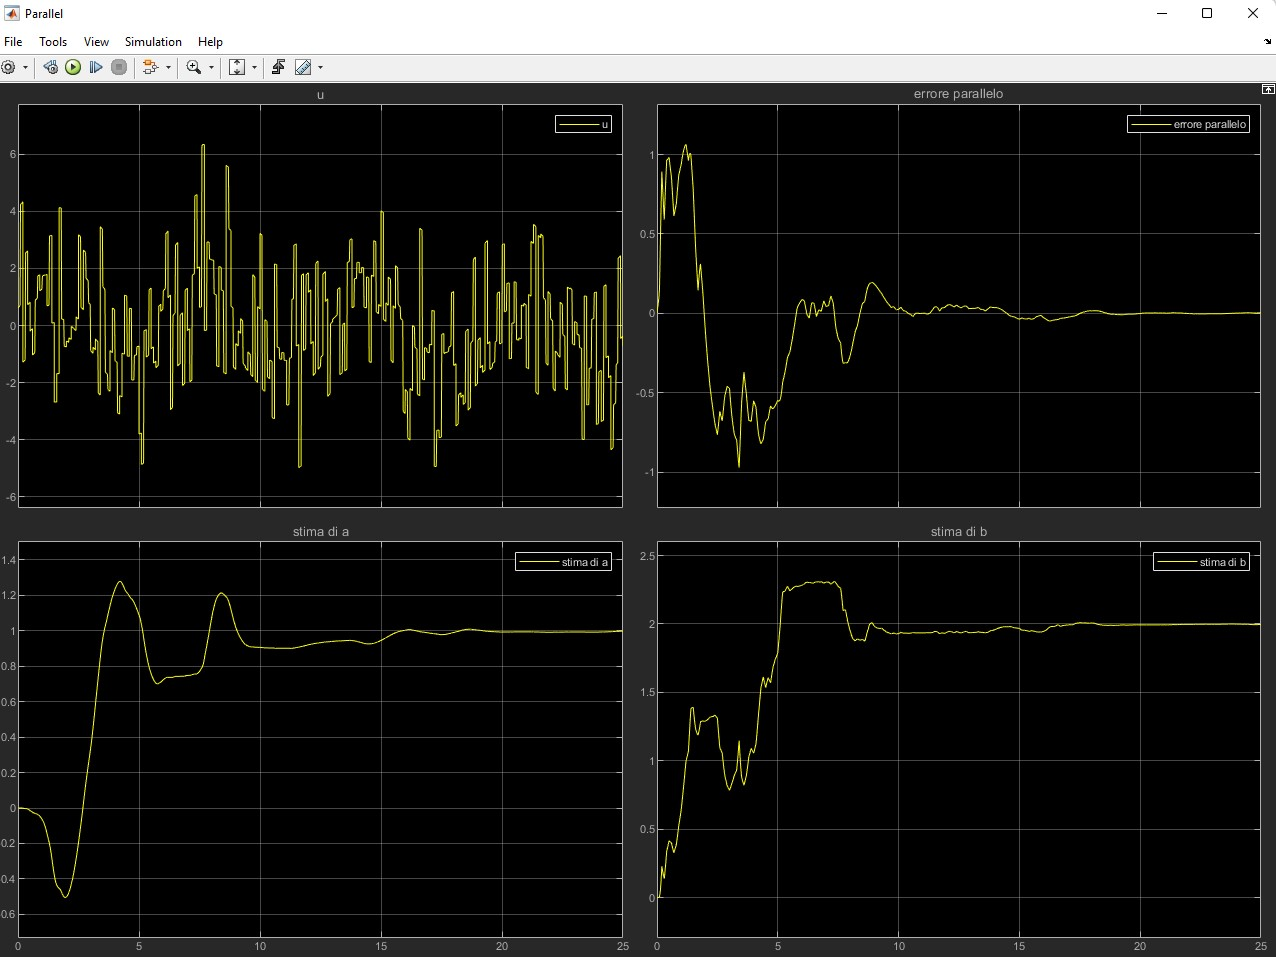
\includegraphics[ scale=0.15]{rumoreInP.jpg}
        &
            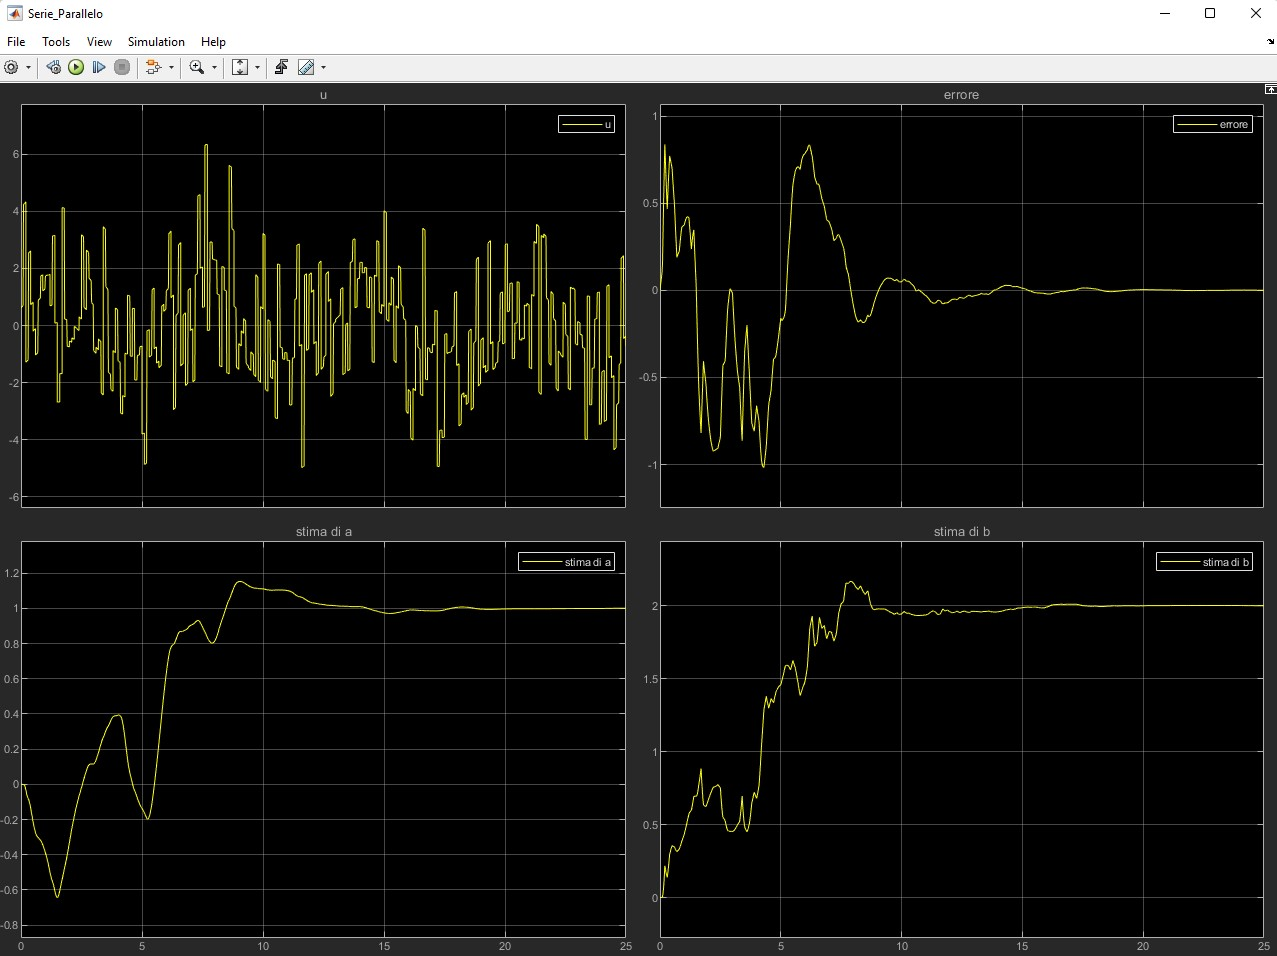
\includegraphics[ scale=0.15]{rumoreInSP.jpg}
        \\
    \end{tabular}\newline
Il rumore in ingresso non impedisce agli algoritmi di stimare i valori dei parametri,ma ne aumenta il tempo di stima dato che l'errore nei primi 10s è molto più altro che in assenza del disturbo.
\end{frame}
\begin{frame}
    \frametitle{Ingresso sinusoidale con rumore sullo stato}
    \subsection{Ingresso sinusoidale con rumore sullo stato}
    \begin{tabular}{cc}
            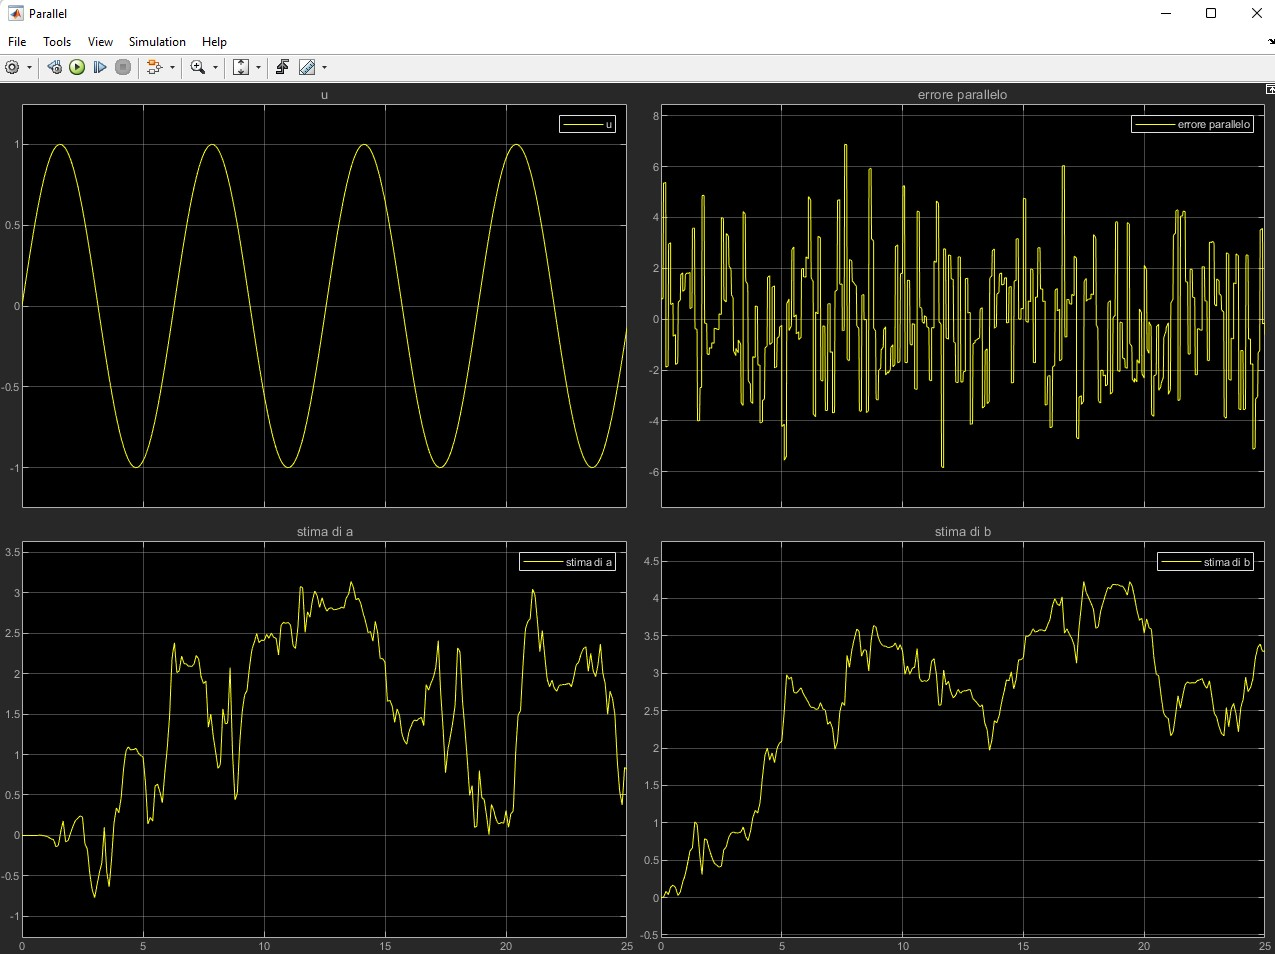
\includegraphics[ scale=0.15]{rumoreXP.jpg}
        &
            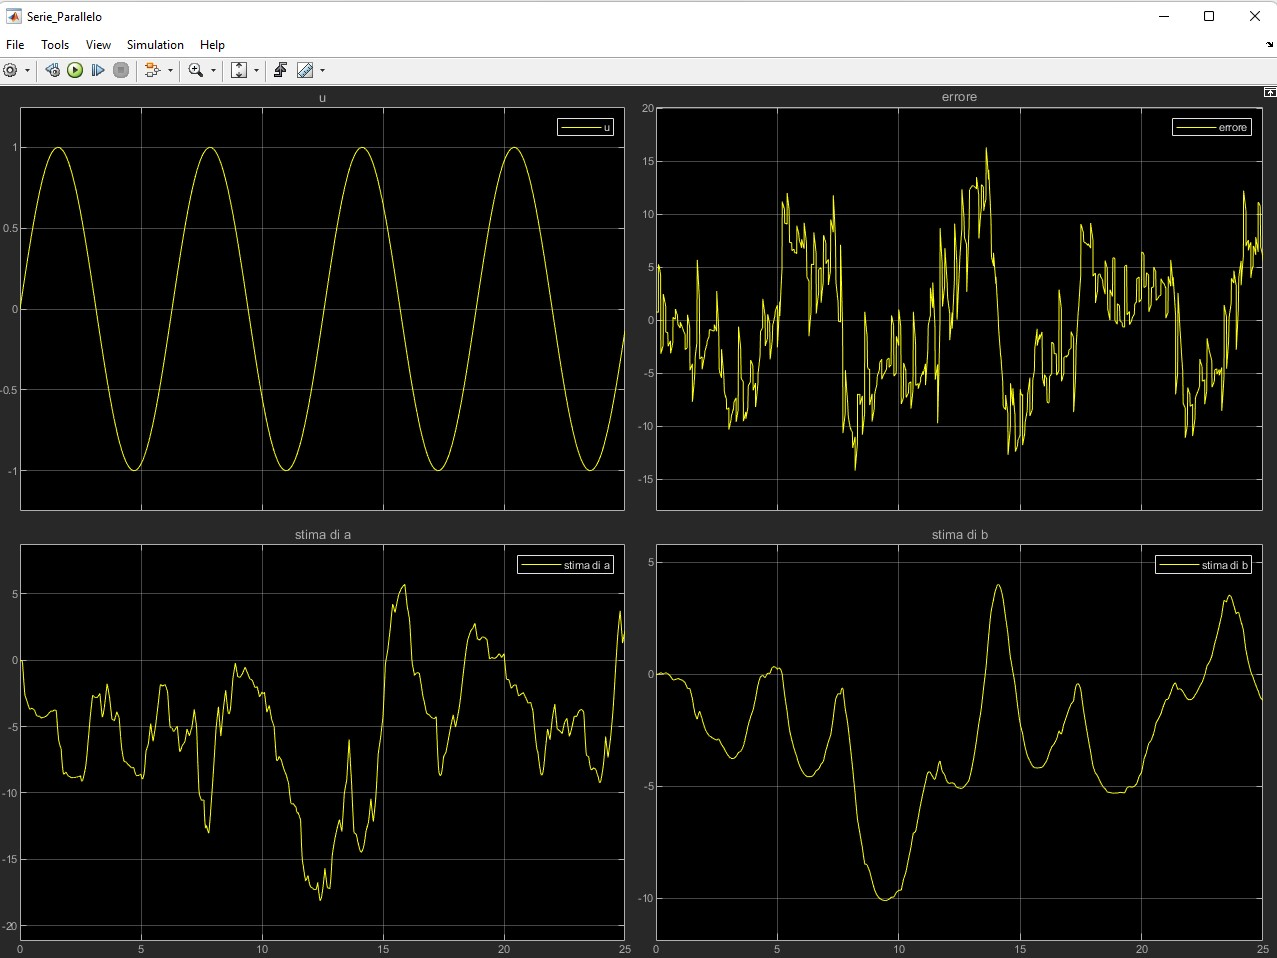
\includegraphics[ scale=0.15]{rumoreXSP.jpg}
        \\
    \end{tabular}\newline
Nel caso in cui ci fosse del rumore sulla misurazione dello stato non sarebbe possibile stimare i parametri del sistema dato che l'errore è pressoché ovunque diverso da 0.
\end{frame}
\begin{frame}
    \frametitle{Variazione del parametro a}
    \subsection{Variazione del parametro a}
    \begin{tabular}{cc}
            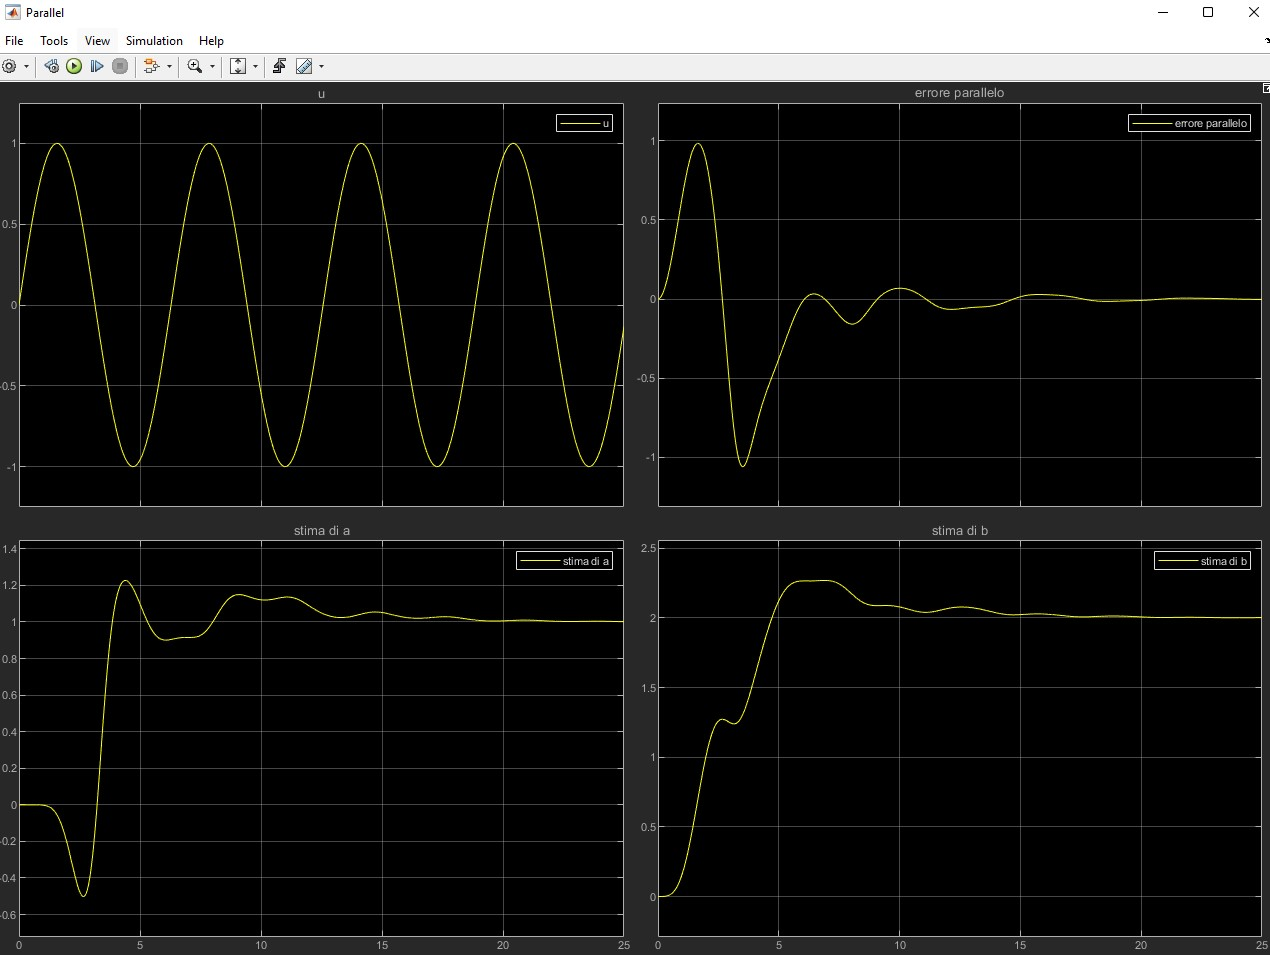
\includegraphics[ scale=0.15]{varaP.jpg}
        &
            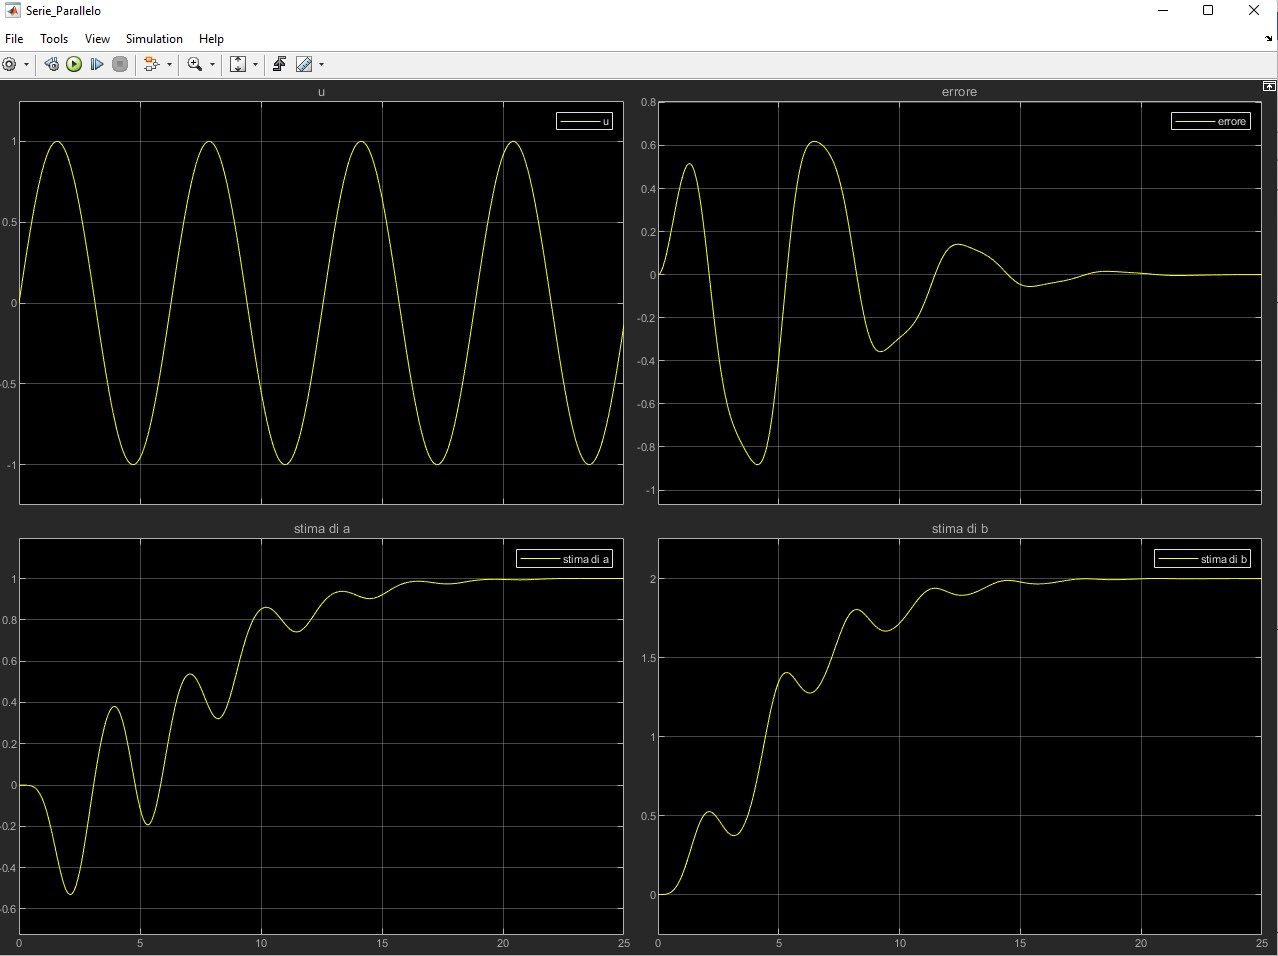
\includegraphics[ scale=0.15]{varaSP.jpg}
        \\
    \end{tabular}\newline
La variazione lenta del parametro a del sistema non causa delle complicazioni agli algoritmi proposti. Nel caso in cui questa variazione è molto rapida e frequente ciò non è più detto.
\end{frame}
\begin{frame}
    \frametitle{Conclusioni}
    \section{Conclusioni}
    Entrambi i modelli consentono di stimare correttamente lo stato rispetto ai vari ingressi. Tuttavia, la soluzione migliore sembrerebbe quella fornita dal modello SP a patto che si conosca bene il sistema e che il bias che viene introdotto sia coerente con quello del sistema.\newline
    Entrambi i modelli soffrono pesantemente sui rumori della misura nello stato, ma a variazioni lente dei parametri del sistema non risentono di queste variazioni.
\end{frame}
\end{document}